\documentclass[tikz, border=1pt]{standalone}

\definecolor{myorange}{rgb}{1, 0.5, 0}

\begin{document}

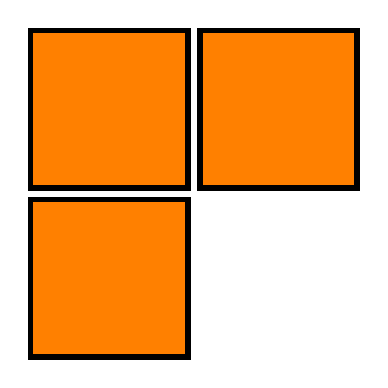
\begin{tikzpicture}[scale=1, line width=2pt]
  % Parameters
  \def\sq{2}      % Square size
  \def\gap{0.15}  % Gap between squares
  % Top Left Square
  \draw[fill=myorange] (0, \sq+\gap) rectangle ++(\sq, \sq);
  % Top Right Square
  \draw[fill=myorange] (\sq+\gap, \sq+\gap) rectangle ++(\sq, \sq);
  % Bottom Left Square
  \draw[fill=myorange] (0, 0) rectangle ++(\sq, \sq);
\end{tikzpicture}

\end{document}
